\chapter{TINJAUAN PUSTAKA}
\label{chap:tinjauanpustaka}

% Ubah bagian-bagian berikut dengan isi dari tinjauan pustaka

Demi mendukung implementasi pada tugas akhir, dasar teori
yang berkaitan akan dijelaskan pada bab ini.
Kajian yang didapat dan dasar teori tersebut
akan digunakan pada tugas akhir ini.

\section{Kubernetes}
\label{sec:kubernetes}

Kubernetes adalah sebuah platform manajemen aplikasi yang dikemas (\emph{containerized applications})
bersifat sumber terbuka. Kubernetes dibuat berdasarkan \emph{tool} internal yang
diciptakan oleh Google bernama Borg untuk mengelola layanan mereka dalam bentuk \emph{container},
kemudian beberapa pengembang Borg menciptakan platform serupa
namun bersifat sumber terbuka yang diberi nama Kubernetes \parencite{borg-references}.

Kubernetes dapat mengelola jalannya aplikasi berbasis kontainer seperti membuat
aplikasi yang tersebut \emph{scalable} dengan cara menambah atau mengurangi \emph{container}
yang menjalankan aplikasi tersebut sesuai dengan kebutuhan pengguna. Untuk memenuhi
hal tersebut, Kubernetes menyediakan beberapa fitur seperti berikut:

\begin{enumerate}
  \item{\emph{Service discovery} dan \emph{load balancing}}
    \par{\emph{Container} pada Kubernetes diekspos oleh Kubernetes menggunakan DNS atau IP dari
      \emph{container} tersebut. Jika \emph{traffic} menuju \emph{container} tersebut tinggi, Kubernetes
      dapat menggunakan \emph{load balancer} agar \emph{deployment} tetap stabil.
    }
  \item{Orkestrasi penyimpanan}
    \par{Kubernetes dapat menggunakan beberapa jenis sistem penyimpanan, seperti
      penyimpanan lokal, penyimpanan dari penyedia jasa \emph{cloud}, dan sebagainya
    }
  \item{\emph{Rollouts} dan \emph{rollbacks} secara otomatis}
    \par{Kubernetes dapat menyesuaikan \emph{state} dari konfigurasi \emph{state} yang
      diberikan, sehingga status dari \emph{state} klaster Kubernetes akan selalu mengikuti
      \emph{state} yang diberikan
    }
  \item{\emph{Self-healing}}
    \par{Kubernetes akan memulai ulang \emph{container} yang gagal atau mati dalam
      mengerjakan \emph{job}, menggantikan \emph{container}, dan akan selalu menunggu
      \emph{container} yang belum siap sebelum pengguna dapat menggunakannya
    }
  \item{\emph{Horizontal scaling}}
    \par{Aplikasi yang di-\emph{deploy} pada Kubernetes dapat di-\emph{scaling} secara
      \emph{horizontal}, yaitu penambahan \emph{Pods} untuk pengerjaan aplikasi tersebut
    }
  \item{IPv4 dan IPv6 \emph{dual-stack}}
    \par{Kubernetes dapat menggunakan IPv4 dan IPv6 untuk alamat IP dari objek dalam Kubernetes
    }
  \item{Desain untuk ekstensibilitas}
    \par{Kubernetes didesain agar mudah dieksten tanpa merubah \emph{source code} dari Kubernetes
    }
\end{enumerate}

\subsection{Arsitektur Kubernetes}

Kubernetes memiliki konsep klaster yang merupakan kumpulan dari satu atau
lebih mesin. Klaster Kubernetes terdiri dari \emph{control plane} yang mengatur
mengatur \emph{worker nodes} dan \emph{Pods} pada klaster
beserta kumpulan mesin \emph{worker} yang disebut sebagai \emph{worker nodes} yang 
menjalankan aplikasi \emph{containerized}. Setiap \emph{cluster} membutuhkan
setidaknya satu \emph{worker nodes} untuk menjalankan \emph{Pods}. Arsitektur
klaster Kubernetes dapat dilihat pada gambar \ref{fig:arsitektur-cluster-kubernetes}

\begin{figure}[H]
  \centering

  % Ubah dengan nama file gambar dan ukuran yang akan digunakan
  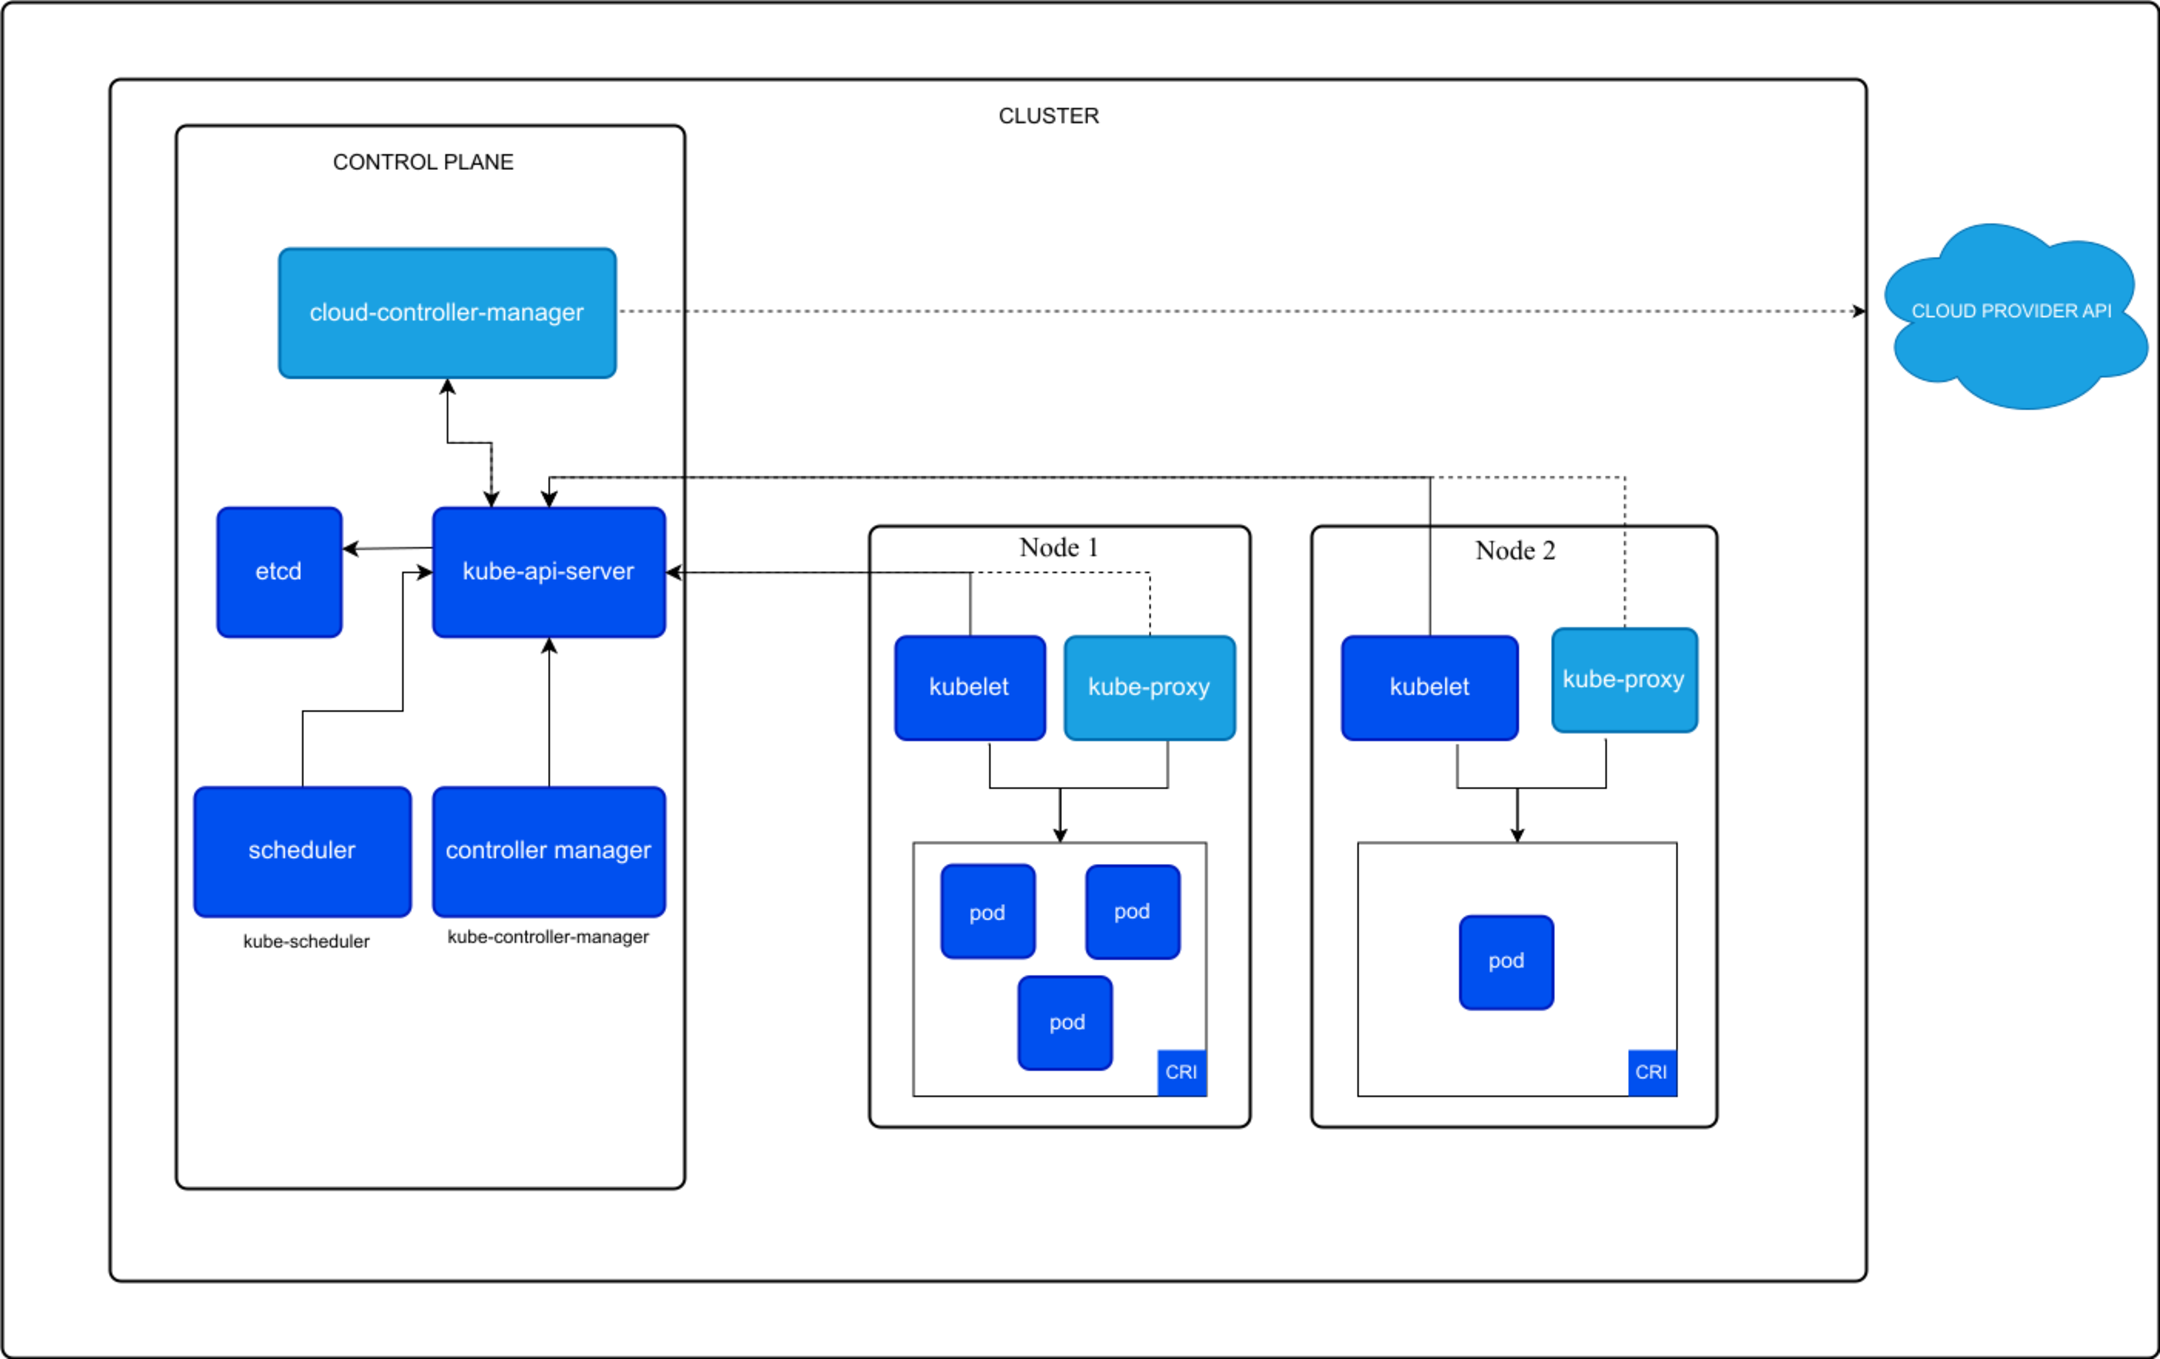
\includegraphics[scale=0.2]{gambar/kubernetes-cluster-architecture.png}

  % Ubah dengan keterangan gambar yang diinginkan
  \caption{Arsitektur klaster Kubernetes}
  \label{fig:arsitektur-cluster-kubernetes}
\end{figure}

\emph{Cluster} tersebut adalah tempat dimana semua \emph{containerized applications},
\emph{jobs}, dan komponen Kubernetes berjalan. 

Untuk membuat \emph{cluster}, Kubernetes memiliki \emph{tool} berupa kubeadm

\subsubsection{Kubernetes Control Plane}

Pada klaster Kubernetes, mesin yang menjadi \emph{control plane} bertugas
untuk membuat keputusan global seperti \emph{scheduling} serta mendeteksi
dan merespon \emph{event} yang terjadi pada klaster tersebut. Untuk melakukan
tugas tersebut, \emph{control plane} memiliki beberapa komponen yaitu kube-apiserver,
etcd, kube-scheduler, kube-controller-manager, dan cloud-controller-manager.

\begin{enumerate}
  
  \item Komponen kube-apiserver berperan sebagai antarmuka dari \emph{control plane}.
    Komponen kube-apiserver melayani komunikasi menggunakan operasi RESTful dan
    mengekspos \emph{shared state} dari klaster yang nantinya digunakan untuk
    interaksi antar komponen.

  \item Komponen etcd merupakan tempat penyimpanan \emph{key-value} secara konsisten.
    Komponen etcd digunakan untuk menyimpan semua data pada klaster seperti \emph{state}
    klaster saat ini dan \emph{state} yang diinginkan.

  \item Komponen kube-scheduler merupakan komponen yang mengamati \emph{Pods} yang telah
    selesai dibuat dan menempatkan \emph{Pods} ke \emph{node} untuk dijalankan. Pada saat
    menempatkan \emph{Pods} ke \emph{node}, kube-scheduler memperhitungkan faktor-faktor
    yang berpengaruh seperti batasan \emph{hardware/software}, kebutuhan sumber daya secara
    individu dan kolektif, spesifikasi afinitas dan non-afinitas, \emph{data locality}, interferensi
    antar beban kerja, dan tenggat waktu dari beban kerja.

  \item Komponen kube-controller-manager berperan untuk menjalankan proses \emph{controller}.
    Proses \emph{controller} mengatur komponen sesuai dengan jenis proses \emph{controller},
    salah satu contohnya adalah proses \emph{node controller} yang mengatur jalannya \emph{node}
    seperti mengamati \emph{node} dan merespon ketika \emph{node} mengalami kegagalan.

  \item Komponen cloud-controller-manager merupakan komponen yang berperan sebagai penghubung
    klaster dengan API khusus dari penyedia layanan awan. Komponen ini memisah
    komponen yang berinteraksi dengan penyedia layanan dan komponen yang hanya berinteraksi dengan
    klaster.

\end{enumerate}

\subsubsection{Kubernetes Node}

Pada sebuah klaster Kubernetes, mesin atau server selain \emph{control plane} akan menjadi \emph{node}.
\emph{Node} bertugas untuk menjalankan \emph{Pods}. Untuk membantu dalam menjalankan tugas tersebut, \emph{node}
memiliki beberapa komponen yaitu kubelet, \emph{container runtime}, dan kube-proxy.

\begin{enumerate}
  
  \item Komponen kubelet merupakan sebuah komponen untuk memastikan \emph{container} berjalan di dalam \emph{Pods}.
    Komponen kubelet menggunakan konfigurasi dari Podspec yang berupa objek YAML atau JSON yang mendeskripsikan
    sebuah \emph{Pods}. Komponen kubelet menerima konfigurasi Podspec yang disediakan dari banyak mekanisme seperti
    apiserver dan memastikan bahwa \emph{container} yang didefinisikan pada Podspec berjalan dengan baik. Komponen kubelet
    tidak mengelola \emph{container} yang tidak diciptakan oleh Kubernetes.

  \item Komponen \emph{container runtime} mengelola \emph{container} pada Kubernetes. Komponen \emph{container runtime}
    bertanggung jawab untuk mengelola \emph{container} seperti eksekusi dan siklus hidup dari \emph{container} yang berjalan
    di lingkungan Kubernetes. Kubernetes mendukung \emph{container runtime} yang mengimplementasikan Kubernetes
    CRI (\emph{Container Runtime Interface}).

  \item Komponen kube-proxy mengatur pengaturan jaringan pada setiap \emph{node}. Pengaturan tersebut mengatur komunikasi
    jaringan menuju \emph{Pods} dari dalam atau luar klaster. Kube-proxy memastikan \emph{request} diteruskan menuju ke
    \emph{container} yang tepat.

\end{enumerate}

\subsection{Objek pada Kubernetes}

Objek pada Kubernetes adalah entitas persisten pada sistem Kubernetes dan digunakan untuk
merepresentasikan keadaan dalam klaster tersebut. Keadaan dalam klaster yang direpresentasikan
oleh objek-objek pada Kubernetes adalah aplikasi yang sedang berjalan pada klaster, \emph{node}
tempat aplikasi berjalan, sumber daya yang tersedia, serta pengaturan kebijakan tentang aplikasi
tersebut.

\subsubsection{Pod}

Pod merupakan unit terkecil yang dapat dibuat dan dikelola pada klaster Kubernetes. Pod sendiri adalah
kumpulan dari satu atau lebih \emph{container} yang berbagi alamat IP dan volume serta
pengaturan mengenai bagaimana \emph{container} tersebut dijalankan. Konfigurasi Pod dapat
diatur dengan konfigurasi deklaratif menggunakan Podspec yang memiliki ekstensi YAML atau JSON.

\subsubsection{test}

\subsection{K3s}

Kubernetes memiliki banyak komponen untuk menjalankan platform Kubernetes. Banyak komponen
tersebut terkadang tidak diperlukan di beberapa skenario. 

K3s merupakan distribusi Kubernetes yang diciptakan oleh Rancher yang
memiliki \emph{size} yang lebih kecil secara keseluruhan. K3s berbentuk
\emph{binary} yang berisi semua \emph{tools} yang dibutuhkan untuk membuat
\emph{cluster} dan bergabung ke \emph{cluster}.

\section{\emph{Multi-tenancy}}
\label{sec:multi-tenancy}

\emph{Multi-tenancy} secara bahasa memiliki arti banyak pengguna atau \emph{tenant}. Dalam konteks
\emph{cloud computing}, \emph{multi tenancy} memiliki definisi pembagian \emph{resource} 
untuk setiap pengguna namun definisi tersebut masih bersifat luas karena implementasi
dari \emph{multi-tenancy} berbeda untuk setiap \emph{service models} \parencite{6830928}.

\section{\emph{Virtual Machine}}
\label{sec:virtual-machine}

\emph{Virtual machine} merupakan lingkungan komputasi terisolasi
yang berjalan di atas mesin fisik. Digagaskan pertama kali oleh IBM
dengan sebuah konsep bernama \emph{time-sharing}. \emph{Time-sharing}
memungkinkan sebuah mesin digunakan oleh lebih dari satu pengguna sehingga
pengguna tersebut terlihat mempunyai sebuah mesin tersendiri.

\begin{figure}[H]
  \centering

  % Ubah dengan nama file gambar dan ukuran yang akan digunakan
  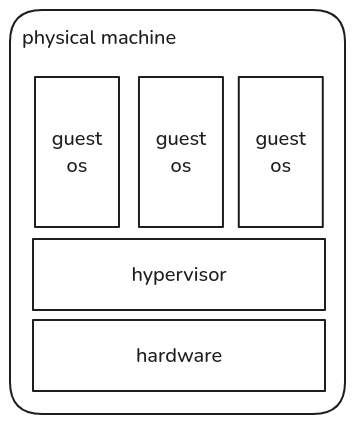
\includegraphics[scale=0.5]{gambar/virtual-machine-architecture.png}

  % Ubah dengan keterangan gambar yang diinginkan
  \caption{Arsitektur \emph{virtual machine}}
  \label{fig:arsitektur-virtual-machine}
\end{figure}

\subsection{QEMU}

QEMU adalah emulator dan virtualisasi mesin generik dan sumber terbuka.

\section{Libvirt}
\label{sec:libvirt}

Libvirt merupakan API untuk berkomunikasi dengan teknologi virtualisasi yang disediakan
oleh sistem operasi.

\section{\emph{Network Bridge}}
\label{sec:network-bridge}

NKASNDLKASNLDASNK

\section{gRPC}

\section{Roket Luar Angkasa}
\label{sec:roketluarangkasa}

% Contoh input gambar
\begin{figure}[H]
  \centering

  % Ubah dengan nama file gambar dan ukuran yang akan digunakan
  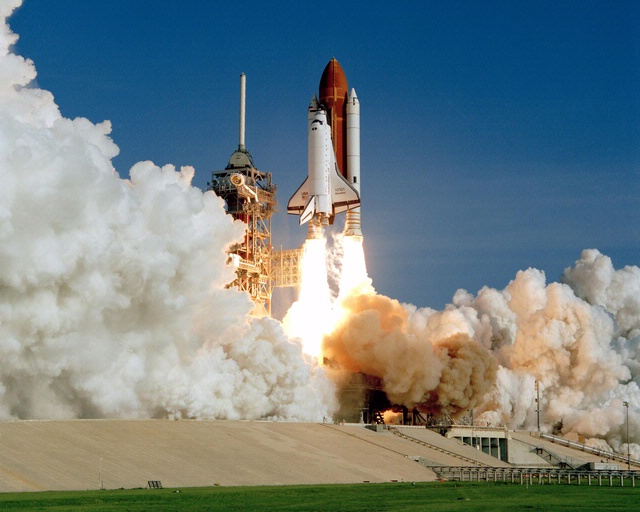
\includegraphics[scale=0.35]{gambar/roketluarangkasa.jpg}

  % Ubah dengan keterangan gambar yang diinginkan
  \caption{Peluncuran roket luar angkasa \emph{Discovery} \parencite{roketluarangkasa}.}
  \label{fig:roketluarangkasa}
\end{figure}

Roket luar angkasa merupakan \lipsum[1]

\emph{Discovery}, Gambar \ref{fig:roketluarangkasa}, merupakan \lipsum[2]

\subsection{Hukum Newton}
\label{subsec:hukumnewton}

Newton \parencite{newton1687} pernah merumuskan bahwa \lipsum[1]
Kemudian menjadi persamaan seperti pada persamaan \ref{eq:hukumpertamanewton}.

% Contoh pembuatan persamaan
\begin{equation}
  \label{eq:hukumpertamanewton}
  \sum \mathbf{F} = 0\; \Leftrightarrow\; \frac{\mathrm{d} \mathbf{v} }{\mathrm{d}t} = 0.
\end{equation}
